\documentclass[dvips,ruledheader]{abnt}
\usepackage[brazil]{babel}
\usepackage[latin1]{inputenc}
\usepackage[pdftex]{graphicx}
\usepackage{abnt-alf}
\usepackage{latexsym}
\usepackage{psfrag}
\usepackage[center]{caption2}

% \newcommand{\lombadassss}{\vec{\mathbf{p}}}

\newcommand{\epigrafe}[1]{
\vspace{1cm}{\raggedright\par\sffamily\slshape #1\par}
}



\newcommand{\lombada}{
\begin{titlepage}
\espaco{1.1}

\begin{center}
	\large\ABNTchapterfont\ABNTautordata
\end{center}

\vspace{7.5cm}

\begin{center}
	\large\ABNTchapterfont\ABNTtitulodata\par
\end{center}

\vfill

\begin{center}
	\textbf{\ABNTlocaldata}\par
	\textbf{\ABNTdatadata}
\end{center}
\end{titlepage}
}


%	Elemento obrigatório, é a cobertura que reveste o trabalho e 
% deve conter informações de identificação da obra, na seguinte ordem (ANEXO AA):
% · nome da instituição (opcional);
% · nome do autor;
% · título;
% · subtítulo (se houver);
% · número de volumes (se houver mais de um, deve constar, em cada capa, 
%  a especificação do respectivo volume);
% · local (cidade) da instituição onde deve ser apresentado;
% · ano de depósito (da entrega).

\newcommand{\mackenzieCapa}{
\begin{titlepage}
\espaco{1.1}

\begin{center}
	\ABNTchapterfont\textbf{\large\MakeUppercase{\ABNTinstituicaodata}}
\end{center}

\vspace{5cm}

\begin{center}
	\large\ABNTchapterfont\MakeUppercase{\ABNTautordata}
\end{center}

\vspace{3.5cm}

\begin{center}
	\large\ABNTchapterfont\MakeUppercase{\ABNTtitulodata}\par
\end{center}

\vfill

\begin{center}
	\textbf{\ABNTlocaldata}\par
	\textbf{\ABNTdatadata}
\end{center}
\end{titlepage}
}

\begin{document}
  \DeclareGraphicsRule{.eps.gz}{eps}{.eps.bb}{`gunzip -c #1}

  % dados da monografia
  \autor{�lvaro Vilobaldo Rios da Silva}
  \titulo{Anti-forense}
  \orientador{Ivete Irene dos Santos}
  \comentario{Monografia da conclus�o do curso de Computa��o forense}
  \instituicao{Universidade Presbiteriana Mackenzie de S�o Paulo}
  \local{S�o Paulo -- SP}
  \data{\today}


  % elementos pr�-textuais
  %	Elemento obrigatório, é a cobertura que reveste o trabalho e 
% deve conter informações de identificação da obra, na seguinte ordem (ANEXO AA):
% · nome da instituição (opcional);
% · nome do autor;
% · título;
% · subtítulo (se houver);
% · número de volumes (se houver mais de um, deve constar, em cada capa, 
%  a especificação do respectivo volume);
% · local (cidade) da instituição onde deve ser apresentado;
% · ano de depósito (da entrega).
\capa
% \mackenzieCapa
  % Lombada
% Elemento opcional, parte da capa do trabalho que reúne as margens internas das folhas,
% sejam elas costuradas, grampeadas, coladas ou mantidas juntas de outra maneira (ANE-
% XO AB).
% Seus elementos devem ser impressos, conforme a NBR 12225:
% · nome do autor(es), impresso longitudinalmente e legível do alto para o pé da lombada;
% · título do trabalho, impresso da mesma forma que o nome do autor;
% · elementos alfanuméricos de identificação, por exemplo: v. 2;
% · ano de depósito (da entrega).

  \folhaderosto
  \include{errata}
  \setlength{\ABNTsignthickness}{0.4pt}
\setlength{\ABNTsignskip}{2cm}


% \begin{folhadeaprovacao}
%   \espaco{1.5}
% 
%   \begin{center}
% 	  \large\ABNTchapterfont\ABNTautordata
%   \end{center}
% 
%   \vspace{5.5cm}
% 
%   \begin{center}
% 	  \large\ABNTchapterfont\ABNTtitulodata\par
%   \end{center}
%   
%   \begin{center}
%       \ABNTcomentariodata
%       
%       Aprovado em: \today 
%       
%       Pelos membros da banca examinadora:
%       \assinatura{\ABNTorientadordata \\ Orientador}
%   \end{center}
%   \vfill
% 
%   \begin{center}
% 	  \textbf{\ABNTlocaldata}\par
% 	  \textbf{\ABNTdatadata}
%   \end{center}
% \end{folhadeaprovacao}


\begin{folhadeaprovacao}

Monografia sob o t\'itulo \ABNTtitulodata , desenvolvida por \ABNTautordata , e aprovada em \today , S\~ao Paulo capital, pela banca constitu\'ida por:
      \assinatura{\ABNTorientadordata \\ Orientador}
\end{folhadeaprovacao}

  \include{dedicatoria}
  \chapter*{Ep�grafe}

\begin{citacao}
  ``Se voc� conhecer o inimigo e a si mesmo, n�o precisa temer o resultado de uma centena batalhas. Se voc� se conhecer a si mesmo, mas n�o o inimigo, para cada vit�ria voc� tamb�m sofrer� uma derrota. Se voc� n�o conhecer nem o inimigo, nem a si mesmo, voc� sucumbir� em todas as batalhas.'' \cite{AGST}
\end{citacao} 


% Sun Tzu (chin�s simplificado: ??; chin�s tradicional: ??; pinyin: S?n W?) (544 a.C. - 456 a.C.) h� mais ou menos 500 anos de cristo j� dizia que se conhecer a si mesmo e ao advers�rio n�o temer� o resultado de mil batalhas.
% 

  % ---------------------------------------------------------------------------------------------------- %
%					ORIENTA��ES
% ---------------------------------------------------------------------------------------------------- %
% Resumo na l�ngua vern�cula
% Elemento obrigat�rio, consiste na apresenta��o concisa dos pontos relevantes do texto.
% Elaborado em portugu�s, p�e em evid�ncia as mat�rias mais importantes do conte�do,
% visando a fornecer, dessa forma, meios para a decis�o do leitor sobre a conveni�ncia, ou
% n�o, de consultar o texto completo.
% Redigido pelo pr�prio autor, contendo de 150 a 500 palavras e deve dar uma vis�o conci-
% sa e clara do conte�do, ou seja, as id�ias principais do texto e as conclus�es do trabalho.
% Na apresenta��o, o resumo deve ser redigido em par�grafo �nico, utilizando-se espa�o
% de 1,5 cm, com frases claras e concatenadas e seguido das palavras mais representati-
% vas do conte�do do trabalho, isto �, palavras-chave e/ou descritores (ANEXO AQ).
% ---------------------------------------------------------------------------------------------------- %


\begin{resumo}
Analisar ambientes comprometidos por rootkits pode representar um verdadeiro desafio e junto com t�cnicas de antiforenses ambos podem criar mecanismos de destrui��o de evid�ncias de forma sistem�tica e eficiente.
Esta monografia � um estudo sobre rootkits e antiforense com a vis�o de um perito computacional forense.
Baseado no funcionamento e premissas do rootkit ser� apresentado um processo para an�lise \emph{post mortem} e as t�cnicas antiforenses em cada uma das suas etapas.

\textbf{Palavras-chave:} antiforense, rootkit, forense, evid�ncias.
\end{resumo}
  \begin{abstract}
This monograph is a study of rootkits and antiforense with the vision of a computer forensics expert.
Based on the premisses and operation of the rootkit is provided a process for analysis \emph{post mortem} and anti-forensic techniques in each of its stages.
Settings antiforense and rootkits with their practices and their common historical along with some techniques of subversion demonstrate that the combined use of techniques antiforenses embedded rootkits engine that creates destruction of evidence in a systematic and efficient.

\textbf{keywords:}  anti-forensics, rootkit, forensics, proof, evidence.
\end{abstract}
  \listoffigures
  % ---------------------------------------------------------------------------------------------------- %
%					ORIENTAÇÕES
% ---------------------------------------------------------------------------------------------------- %
% Lista de tabelas
% Elemento opcional, elaborada de acordo com a ordem apresentada no texto, com cada
% item designado por seu nome específico, acompanhado do respectivo número da página
% (ANEXO AV).
% ---------------------------------------------------------------------------------------------------- %

\listoftables
  \include{abreviaturas}
  \tableofcontents 

  % elementos textuais
  % ---------------------------------------------------------------------------------------------------- %
%					ORIENTA��ES
% ---------------------------------------------------------------------------------------------------- %
% 	� a apresenta��o sucinta e objetiva do trabalho, fornecendo informa��es sobre sua natu-
% reza, import�ncia e crit�rios de elabora��o, tais como: objetivos, m�todos e procedimen-
% tos seguidos.
% Lendo a introdu��o, o leitor deve sentir-se esclarecido a respeito do conte�do do trabalho,
% assim como do racioc�nio que foi desenvolvido.
% ---------------------------------------------------------------------------------------------------- %

\chapter{Introdu��o}

% ---------------------------------------------------------------------------------------------------- %
%					ORIENTA��ES
% ---------------------------------------------------------------------------------------------------- %
%	Na introdu��o voc� deve retomar os itens do projeto e deixar bem claros: tema, objetivos, 
% justificativa, metodologia e se poss�vel, quais ser�o os cap�tulos, ou seja, comentar o sum�rio, 
% apresnetando o que far� em cada cap�tulo.
% ---------------------------------------------------------------------------------------------------- %

O rootkit � uma ferramenta utilizada em geral por atacantes avan�ados com fins maliciosos e oferece grande obst�culo para ser detectado justamente por ser furtivo e sofisticado recurso de controle de sistemas operacionais.
Seu uso for�a o perito a ter um conhecimento amplo e usar t�cnicas tamb�m sofisticadas para investiga-lo.
Logo entender o seu funcionamento � determinante para uma pericia bem sucedida. 

Esta monografia apresenta uma incurs�o na antiforense focada na utiliza��o de rootkits em ambientes \emph{Microsoft Windows}, visando mostrar o que � um rootkit e os principais empecilhos que o perito pode encontrar ao analis�-lo. 
Para desenvolver esse tema foi utilizada vasta bibliografia e refer�ncias reais para melhor entendimento das t�cnicas de antiforense computacionais utilizadas ou idealizadas que podem ser utilizados por rootkits.

\section{Justificativa}

% ---------------------------------------------------------------------------------------------------- %
%					ORIENTA��ES
% ---------------------------------------------------------------------------------------------------- %
% 	Na justificativa busca-se colocar, de maneira clara e objetiva, quais s�o os elementos 
% te�rico-pr�ticos que demonstram a relev�ncia para a realiza��o da pesquisa, bem como as poss�veis 
% contribui��es resultantes do trabalho proposto.
% ---------------------------------------------------------------------------------------------------- %

Conforme o mundo digitalizou-se, digitalizaram-se tamb�m as suas amea�as, onde antes se podia ver mesmo que por instantes m�sseis ou bombas sendo lan�ada hoje temos in�meras amea�as invis�veis que podem causar tanto estrago quanto, contudo na luz do princ�pio de Locard que diz que tudo que � tocado deixa vest�gios, talvez essas amea�as n�o sejam t�o invis�veis.
O perito deve estar preparado para a a��o de um usu�rio avan�ado que conhe�a bem o sistema operacional atacado, comprometido ou usado.
Mesmo que n�o seja algo corriqueiro na rotina da grande maioria dos profissionais, encontrar um atacante de alto n�vel trar� novos desafios e obst�culos t�o pouco corriqueiros quanto.
Saber como dificultar ou impossibilitar o trabalho do perito � como ele poder� evitar a armadilha de achar que no corpo (corpo de delito) investigado n�o existe nada.

A figura \ref{fig:graph-root} mostra que quantidade de amostras �nicas encontradas de rootkits entre 2009 e 2012 por trimestre nunca foi abaixo de 100 mil.
Esses dados indicam que rootkits s�o amea�as reais e constantes. 
Estudar seu comportamento e entender como ele pode ser usado na antiforense, permite ao perito lidar corretamente com rootkits.

\begin{figure}[htb]
  \centering
  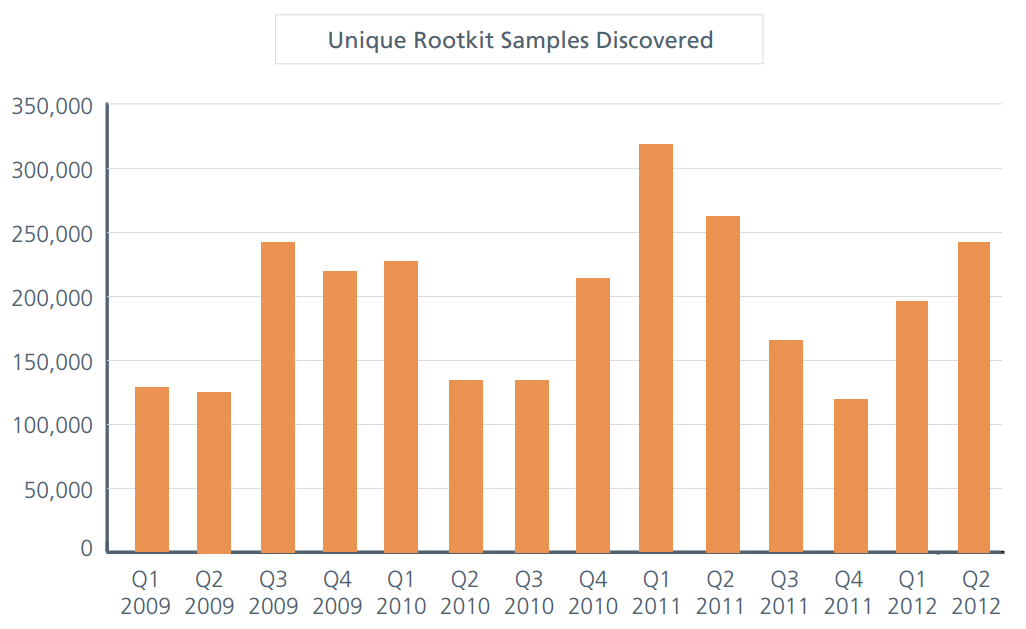
\includegraphics[scale=0.5]{figuras/graph-root.png}
  \caption{Amostras Rootkit �nicas Descobertas \cite{MCAFEE2012}}
  \label{fig:graph-root}
\end{figure}

Com um processo bem definido o perito tende a diminuir o tempo de an�lise e um melhor aproveitamento das mesmas.
Sendo assim, esse trabalho poder� ajudar a tra�ar um processo bem elaborado de trabalho que seja r�pida e eficiente sem deixar brechas que permitam ou ajudem a��es antiforenses provendo mais qualidade com mais precis�o.

\section{Objetivos}

% ---------------------------------------------------------------------------------------------------- %
% Que problemas o estudo do tema pode resolver? (PREPARA��O PAR AO PROBLEMA DE PESQUISA E OBJETIVO)}
% ---------------------------------------------------------------------------------------------------- %

Esse estudo pode ajudar a esclarecer diversos t�picos obscuros a respeito do que pode ser encontrado em investiga��es forenses computacionais quando o perito se v� diante de amea�as persistentes e elaboradas como um rootkit e consequentemente pode ajudar a resolver casos onde foram feitas antiforense.

\subsection{Objetivo Geral}

% ---------------------------------------------------------------------------------------------------- %
%					ORIENTA��ES
% ---------------------------------------------------------------------------------------------------- %
%	� necess�rio apresentar o objetivo geral da pesquisa, ou seja, a meta proposta para a investiga��o, 
% que deve ser coerente com a quest�o de pesquisa.
% ---------------------------------------------------------------------------------------------------- %

Apresentar um processo para an�lise \emph{post mortem} de computadores com Microsoft Windows e as principais t�cnicas antiforense que podem ser encontradas em cada fase do processo.

\subsection{Objetivo Espec�fico}

% ---------------------------------------------------------------------------------------------------- %
%					ORIENTA��ES
% ---------------------------------------------------------------------------------------------------- %
%	De forma complementar, os objetivos espec�ficos, tamb�m presentes nesse item, constituem as etapas 
% de trabalho que permitem alcan�ar o objetivo geral. Como os objetivos traduzem a��es que ser�o executadas 
% ao longo da pesquisa; a apresenta��o destes no texto requer a utiliza��o de verbos no infinitivo.
% ---------------------------------------------------------------------------------------------------- %
Segue os objetivos espec�ficos utilizados para alcan�ar o objetivo principal:

\begin{itemize}
  \item Apresentar o que � ci�ncia forense, para que serve a ci�ncia forense e a legisla��o que garante a exist�ncia do perito no Brasil;
  \item Expor o que � um rootkit, seu funcionamento e seus tipos;
  \item Mostrar o que � antiforense computacional categorizando seus tipos; e
  \item Apresentar um processo de an�lise de rootkit.
\end{itemize}
 
\section{Descri��o dos Cap�tulos}

Ao longo dos cap�tulos s�o desenvolvidos os conhecimentos para o entendimento do tema proposto, onde cada um foi dividido em um assunto espec�fico.

No cap�tulo \emph{Ci�ncia Forense Computacional}, ser� mostrado uma vis�o geral do que � a ci�ncia forense, como ela � aplicada na computa��o, o que � um perito forense computacional e o respaldo legal para sua atua��o.

No cap�tulo \emph{Rootkit}, conduz a uma vis�o do funcionamento de um rootkit, algumas t�cnicas para subverter os sistema, o que � um \emph{malware}, a origem do nome rootkit, o que significa ser o usu�rio \emph{root}, os objetivos do rootkit, suas premissas e sua defini��o.
Tamb�m ser� mostrado os tipos de rootkits e analisado duas categorias gerais que exemplificam como o rootkit pode se manter oculto.

Por fim no �ltimo cap�tulo \emph{An�lise de Rootkits}, ser� apresentado um processo de an�lise \emph{post mortem} com passos que ir�o mostrar em cada etapa o que deve ser feito, t�cnicas antiforense e o qu�o complicado e impactante ela �.

% \section{Metodologia}
% \section{descricao dos capitulos} 

%Peritos em sua nobre luta di�ria podem se deparar, em uma das suas pr�ximas empreitadas t�o ut�is para a sociedade, com algum artefato que tenham sido subvertido por algu�m com o mesmo ou um maior conhecimento do que o seu sobre o corpo de delito periciado.

%Portando em assuntos que fojem da mediocridade cotidiana e adentram nesse mundo instigante e revelador da an�lise de artefatos �nicos, se faz necess�rio que quanto maior o desafio, maior dever� ser a dedica��o e paix�o do perito.

% O perito deve precaver-se de supor que situa��es mais corriqueiras tenham s� e apenas a resposta mais obvia desse modo evitando que sejam subestimadas.
% Al�m do conhecimento t�cnico e de foro que se espera de um perito, compreender que existem t�cnicas sofisticadas para destruir e/ou dificultar acesso a provas no ambito computacional � de fundamental necessidade para qualquer perito. 
% A combina��o do uso de diversas t�cnicas avan�adas com maestria se mostra realmente desafiadora, pois quando isso ocorre o artefato investigado pode estar preparado para ser investigado removendo rastros e evitando a cri��o de evid�ncias.
  \include{desenvolvimento}
  \chapter{Conclusão}
nao existe tecnica antiforense 100\% nem metodologia para analise infalivel, nem 100\% segura e confiavel. foi mostrado diversas técnicas para atrasar e confundir o perito, e por vezes tornando o tempo de análise tao grande que o mesmo nao poderia 


  % elementos p�s-textuais
  \bibliography{bb}
\bibliographystyle{abnt-alf}
  \include{glossario}
  \include{apendiceanexos}

\end{document}
